\documentclass[nohyperref]{article}
\usepackage[utf8]{inputenc}
\usepackage{amsmath}
\usepackage{amssymb}
\usepackage{color}
\usepackage{tikz, pgfplots}
\usepackage{pgfplotstable}
\pgfplotsset{compat=1.17}
\usetikzlibrary{shapes,arrows,calc,trees,positioning}
\usetikzlibrary{chains,fit,shapes.geometric}

\begin{document}

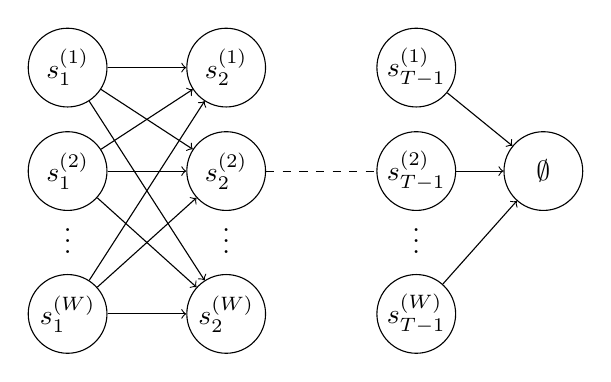
\begin{tikzpicture}[main/.style = {draw, circle, minimum size=1cm}] 
\node[main, label=center:$s_1^{(1)}$] (11) {}; 
\node[main, label=center:$s_1^{(2)}$] (12) [below=0.3cm of 11] {}; 
\node (ellipsis1) [below=1.2cm of 11] {$\vdots$};
\node[main, label=center:$s_1^{(W)}$] (1w) [below=0.8cm of 12] {}; 

\node[main, label=center:$s^{(1)}_2$] (21) [right=1cm of 11] {}; 
\node[main, label=center:$s^{(2)}_2$] (22) [right=1cm  of 12] {}; 
\node (ellipsis2) [below=1.2cm of 21] {$\vdots$};
\node[main, label=center:$s^{(W)}_2$] (2w) [right=1cm  of 1w] {}; 



\node[main, label=center:$s^{(1)}_{T-1}$] (d1) [right=1.4cm of 21] {}; 
\node[main, label=center:$s^{(2)}_{T-1}$] (d2) [right=1.4cm of 22] {}; 
\node (ellipsisd) [below=1.2cm of d1] {$\vdots$};
\node[main, label=center:$s^{(W)}_{T-1}$] (dw) [right =1.4cm of 2w] {}; 

\node[main, label=center:$\emptyset$] (end) [right=0.6cm of d2] {};

 
\draw [->] (11) -- (21);
\draw [->] (12) -- (21);
\draw [->] (1w) -- (21);

\draw [->] (11) -- (22);
\draw [->] (12) -- (22);
\draw [->] (1w) -- (22);

\draw [->] (11) -- (2w);
\draw [->] (12) -- (2w);
\draw [->] (1w) -- (2w);








\draw [->] (d1) -- (end);
\draw [->] (d2) -- (end);
\draw [->] (dw) -- (end);

\draw[dashed] (22) -- (d2);

\end{tikzpicture}

\end{document}